
\begin{itemize}
	
	\item Comment on calcul $\phaseg$ en pratique ?
	
	\item Application
	
	\item Conclusion sur le mémoire et perspective.
\end{itemize}




\section{Calcul pratique de la phase géométrique}

Dans la \cref{part:phase_geo} précédente, deux formulations de la phase géométrique ont été présentées. Cela dit, elles ne sont que très peu pertinentes pour le calcul de $\phaseg$ en pratique car passant par des intégrales dans $\PC{n}$ qui ne s'écrivent explicitement qu'avec des coordonnées locales.
\\

Une solution apporté par Rabei \etal~\cite{rabei_bargmann_1999} est de s'intéresser à une approximation polygonale du signal projeté dans $\PC{n}$. 
C'est-à-dire de l'approcher par une suite de géodésiques concaténées les unes aux autres. 
\\
Sachant que les mesures sont toujours de nature discrète, cette opération n'a pas vraiment de coût en pratique et permet d'exploiter les résultats de la \cref{part:phase_geo}, \cref{subsec:phase_g2geode}. 
Ainsi, en notant $(\x_i)_{1\leq i\leq k}$ les $k$ mesures du signal, $\x_{i\rightarrow i+1}$ la géodésique reliant $\x_i$ à $\x_{i+1}$, et $\x$ la concaténation de toutes ces géodésiques, on a  :


\begin{wrapfigure}[10]{r}{0.43\textwidth}
	\fbox{\begin{minipage}{18em}
			\vspace{0.3cm}
			\begin{algorithmic}[0]
				\State $(\x_n)_{0\leq n\leq N}$ : signal
				\State $\x\ \longleftarrow\ 2\iFou{\one_{\R^+}\Fou{\x}}$ 
				\State
				\State $\phaset = 0$ : phase totale
				\State $\phased = 0$ : phase dynamique 
				\State $\phaseg = 0$ : phase géométrique
				\State 
				\For{$n\in \llbracket1,N\rrbracket$}
				\State $\phaset\ \longleftarrow\  \arg\langle\x_n, \x_1\rangle$
				\State $\phased\ \longleftarrow\  \phased + \arg\langle\x_n, \x_{n-1}\rangle$
				\State $\phaseg\ \longleftarrow\  \phaset - \phased$
				
				\Return $\phaset$, $\phased$, $\phaseg$
				\EndFor
			\end{algorithmic}
			\vspace{0.2cm}
	\end{minipage}}
	\caption{Pseudo-code du calcul des trois phases sur tout un signal $\x$, avec transformation en SA.}
	\label{fig:p-code_calc_phases}
\end{wrapfigure}

\par \noindent
\begin{align*}
	\phaseg(\x) &= \phaset(\x) - \phased(\x) \\
	&= \phaset(\x) - \sum_{i=1}^{k-1} \phased(\x_{i\rightarrow i+1}) \\
	&= \phaset(\x) - \sum_{i=1}^{k-1} \phaset(\x_{i\rightarrow i+1}) - \phaseg(\x_{i\rightarrow i+1}) \\
	&= \phaset(\x) - \sum_{i=1}^{k-1} \phaset(\x_{i\rightarrow i+1}) \\
	&= \arg\langle\x_k, \x_1\rangle - \sum_{i=1}^{k-1} \arg\langle\x_{i+1}, \x_i\rangle
\end{align*} 
\\
Cette formule, en plus d'être facilement implémentable, n'est que très peu coûteuse en temps de calcul. *
Aussi, elle est partiellement itérative, permettant d'obtenir un algorithme de calcul de $\phaseg$ en tout point relativement efficace (\cf~\cref{fig:p-code_calc_phases}). 
C'est cette formule qui est implémentée dans les codes disponibles sur le \href{https://github.com/GregoireDoat/StageM2}{GitHub}.
\\



\section{Première application : ondes gravitationnelles} \label{subsec:ex-3D}

En relativité générale, la gravité n'est plus décrite comme une force mais comme une conséquence de la déformation de la métrique de l’espace-temps en fonction des masses qui s'y trouvent \cite{vankov_einsteins_nodate}.
Cela a de multiples conséquences, comme par exemple le fait que la lumière puisse être déviée par les objets massifs, ce qui ne pouvait pas être le cas en mécanique Newtonienne et qui fût confirmé expérimentalement.
\\
Une autre prédiction de la relativité générale est l'existence d'onde gravitationnelle, qui sont dues à la propagation des déformations de l’espace-temps causées par le déplacement d’objet massif.
Cela dit, mesurer de telles ondes n'est pas chose aisée et il a fallu attendre cent ans après l'article fondateur d'Einstein (1915) pour pouvoir les détecter (2015).
\\

En plus de leur existence, la théorie de la relativité générale prédit que ces ondes doivent être polarisées, comme ça peut être le cas avec les ondes électromagnétiques ou sismiques. En revanche, il n'a pas encore été possible de confirmer que nos mesures présentent effectivement ces propriétés, que ce soit dû au niveau de bruit élevé des mesures ou à des difficultés techniques au niveau des capteurs. Mettre en évidence ces propriétés serait une validation expérimentale supplémentaire de la théorie d'Einstein et sur ce point la phase géométrique est un outil prometteur.
\\

Avant d'y venir, revenons sur les mesures. Pour pouvoir détecter des ondes aussi discrètes, il est nécessaire de se tourner vers des objets à la fois massifs et en mouvement rapide, en l'occurrence des systèmes binaires de trous noirs (BBH, Binary Black Holes) en phase de ``merge''. C'est-à-dire deux étoiles massives, ici des trous noirs, en orbite l'une autour de l'autre et sur le point d'entrer en collision, comme le montre la \Cref{fig:merge2BBH} ci-dessous :

\begin{figure}[h]
	

\begin{floatrow}
	
	\ffigbox[0.5cm]{}
	{{\color{white}tobin}}
	
	\ffigbox[4cm]{}
	{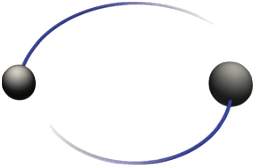
\includegraphics[height=1.75cm]{fig/not_mine/imr_i1.png}}
	
	\ffigbox[4cm]{}
	{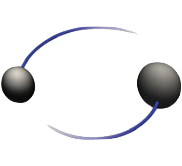
\includegraphics[height=1.75cm]{fig/not_mine/imr_i2.png}}
	
	\ffigbox[2cm]{}
	{
\includegraphics[height=1.75cm]{fig/not_mine/imr_m.png}}
	
	\ffigbox[2cm]{}
	{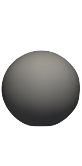
\includegraphics[height=1.75cm]{fig/not_mine/imr_r.png}}
\end{floatrow}

\begin{floatrow}
	\ffigbox[0.9\textwidth]{\caption[Différentes étapes de la fusion de deux trous noir]{Différentes étapes de la fusion de deux trous noirs. Figure tirée de {\normalfont \cite[fig. 4]{flores_damped_nodate}}.} \label{fig:merge2BBH}}
	{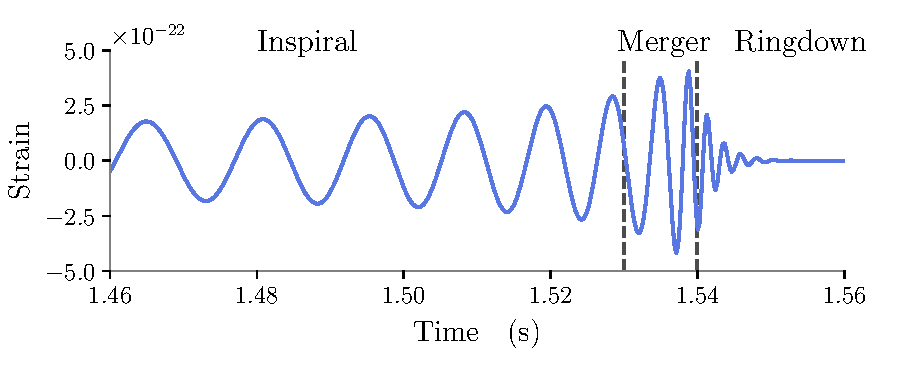
\includegraphics[width=0.9\textwidth]{fig/not_mine/inspiral_merger_ringdown.pdf}}
\end{floatrow}
\end{figure}

Il est donc prédit que les ondes engendrées par ces phénomènes sont polarisées mais aussi, et surtout, qu'en fonction de l'alignement des axes de rotations des deux étoiles, l'état de polarisation de ces dernières doit varier au cours du temps. Chose qui doit pouvoir être mise en évidence par le calcul de la phase géométrique des ondes.
\\

Pour cela, sont utilisés quatre jeux de données synthétiques et sans bruit avec des axes de rotations plus ou moins alignés et la \Cref{fig:phase_g2GW} présente l’évolution des trois phases du signal dans chacun des cas.
\\
\begin{figure}[h]
	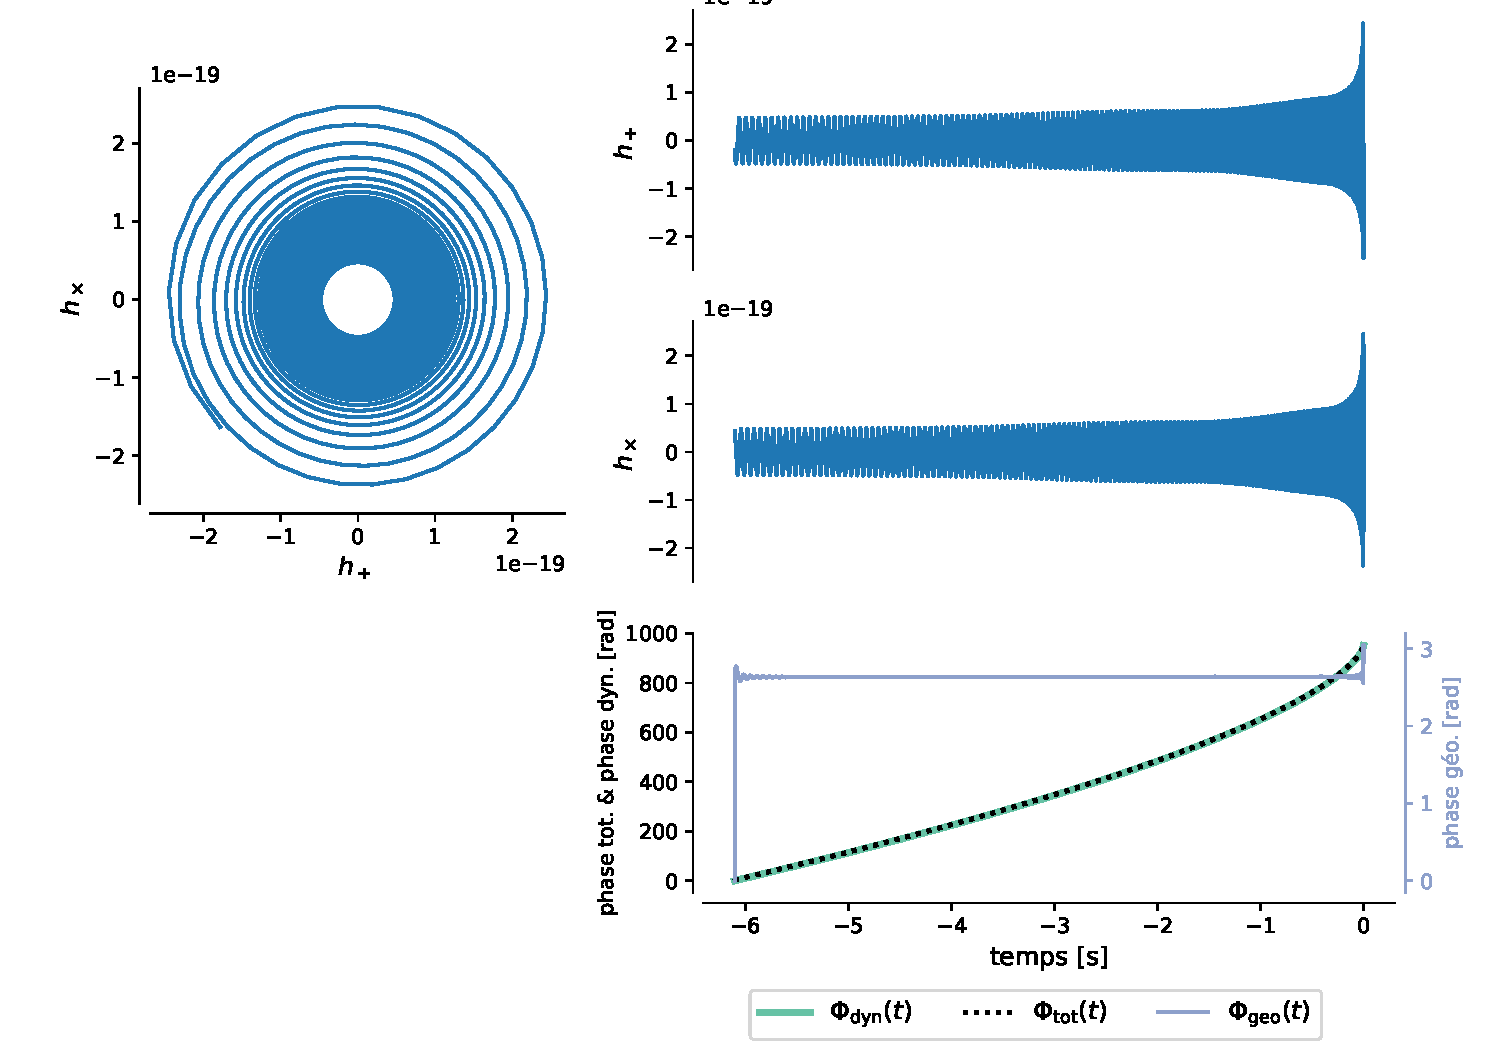
\includegraphics[width=0.5\textwidth]{fig/part-3/GW_plot_1.pdf}\hfill
	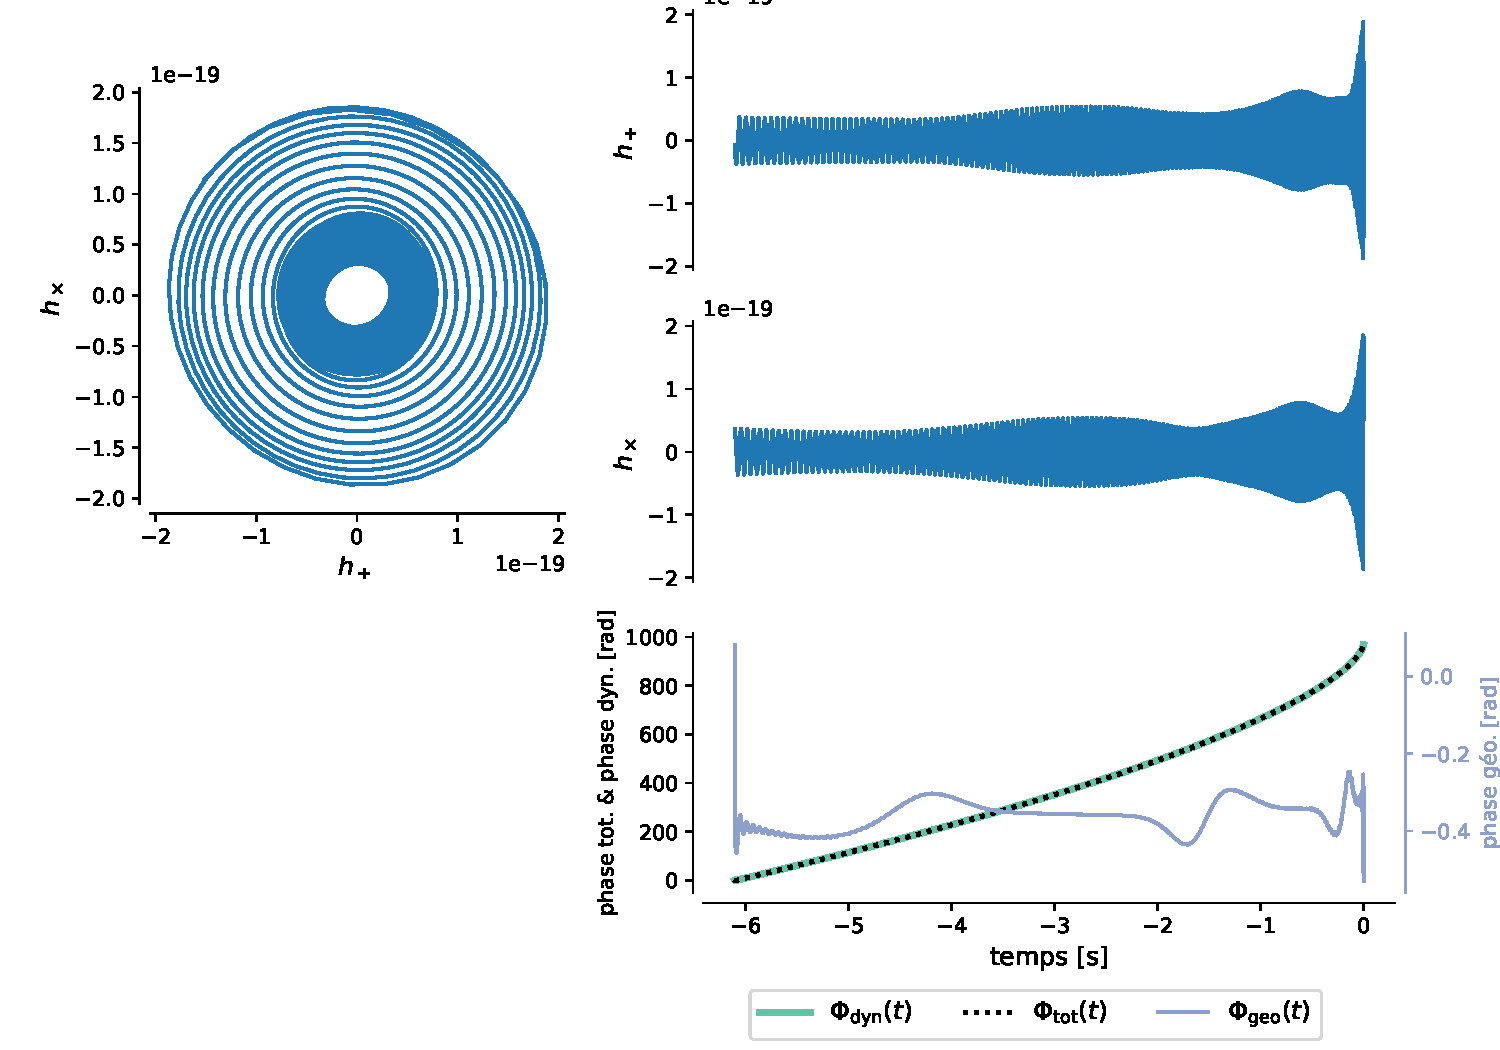
\includegraphics[width=0.5\textwidth]{fig/part-3/GW_plot_2.pdf}\\
	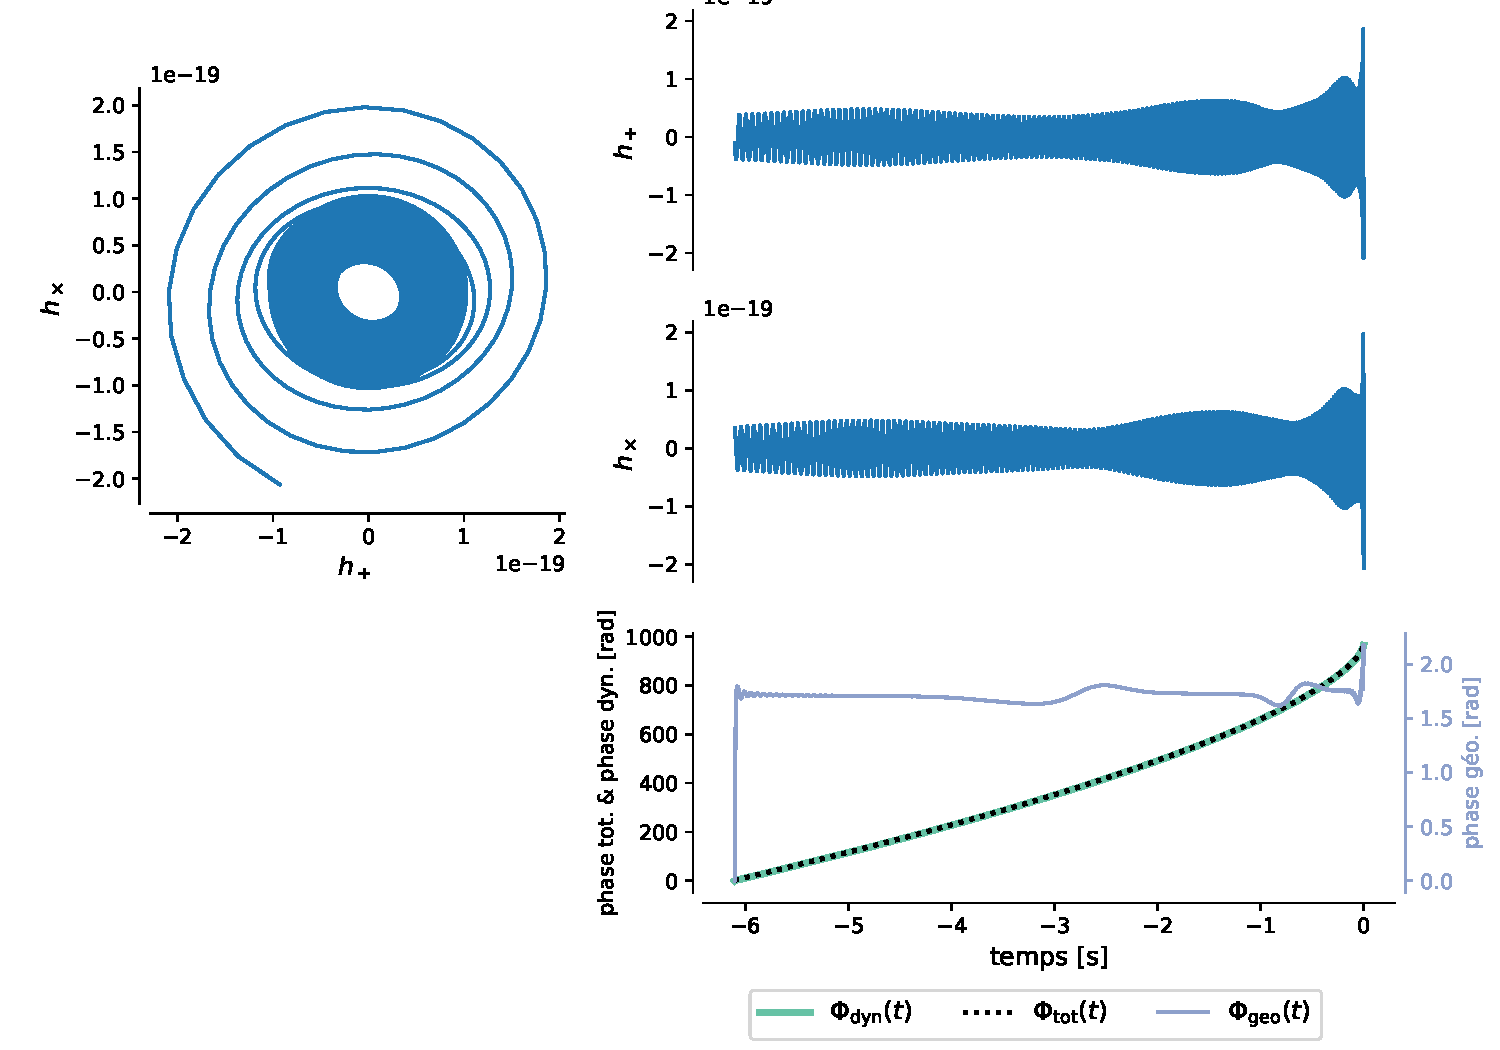
\includegraphics[width=0.5\textwidth]{fig/part-3/GW_plot_3.pdf}\hfill
	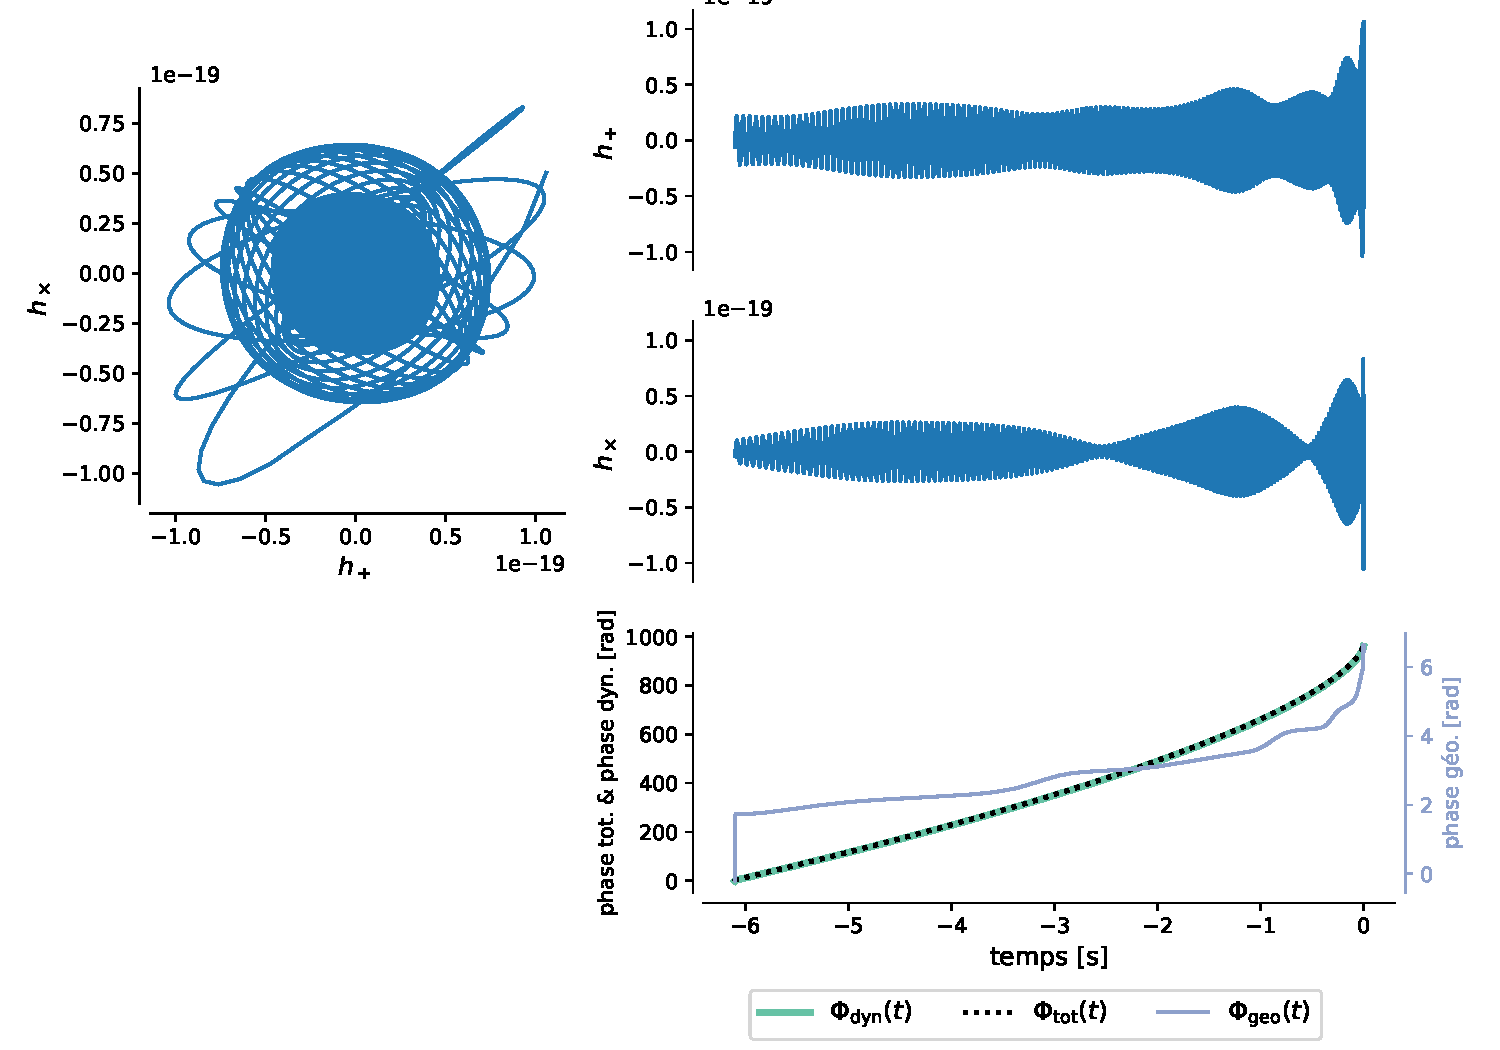
\includegraphics[width=0.5\textwidth]{fig/part-3/GW_plot_4.pdf}
	\caption[Évolution de la phase géométrique sur des données simulées d'ondes gravitationnelles]{Évolution de la phase géométrique sur des données simulées d'ondes gravitationnelles. Sur chaque graphique (de haut en bas et de gauche à droite) les spins des trous noirs sont de moins en moins alignés. Dans les parties hautes sont représentés les signaux simulés et, en dessous, le calcul des différentes phases.}
	\label{fig:phase_g2GW}
\end{figure}

Ces signaux étant à valeurs dans $\R^2$, il a fallu les transformer en signaux analytiques pour pouvoir calculer leurs différentes phases. Cela suppose (\cf~\ref{ann:complement_t-f}) qu'ils soient de type AM-FM-PM, ce qui n'est pas un problème au vu de l'allure des composantes $h_+$ et $h_\times$ des signaux.
\\
Ensuite, comme attendu, la phase géométrique de ces signaux n'est pas constante et devient de plus en plus changeante à mesure que la polarisation des ondes devient variable.
\\

Ces résultats, bien que très préliminaires, permettent déjà d'entrevoir les difficultés quant à la mesure de la phase géométrique :
\\
D'abord, au début de chaque signal, elle présente un saut conséquent par rapport à ses valeurs et il semblerait qu'il soit très sensible à la valeur de départ du signal. Aussi, quand bien même ce saut ne semble pas se faire d'un multiple de $\pi$, il est probable que ce soit en partie lié au choix de représentant de $\phaseg$ (qui est définie modulo $2\pi$).
Dans tous les cas, cela risque de poser problème pour une utilisation plus avancée.
\\
Ensuite, même dans le pire des cas, la phase géométrique ne reste que très marginale par rapport aux deux autres, ce qui risque d'être un problème sur des mesures réelles, nécessairement bruitées.
\\




\section{Conclusion et perspectives}

Même si ce n'était pas l'objectif premier, s’intéresser à la phase géométrique a permis d'apporter un point de vue nouveau sur les signaux multivariés en terme de paramètres instantanées (amplitude, phase et polarisation). 
\\
Cela a permis, d'un côté, de mettre en lumière une subtile limite du modèle AM-FM-PM au niveau de l'interprétabilité de ces paramètres $(\varphi, \theta, \chi)$ et pourquoi il était nécessaire de passer par des notions de géométrie différentielle pour retrouver ces interprétations. 
De l'autre, cela a permis de donner une nouvelle interprétation, en terme de signal, à des outils déjà bien connus en mécanique quantique.
\\

Il a été montré que la phase géométrique est une quantité qui se mesure effectivement en pratique et, même si ces interprétations géométriques laissent entendre que ses applications sont limitées, il n'est pas exclu qu'elle puisse avoir des applications en débruitage. Par exemple, si une onde mesurée n'est pas censée être à polarisation variable, une phase géométrique non nulle de ce dernier ne pourrait être due qu'à du bruit. On pourrait alors imaginer des traitements qui se feraient uniquement sur le signal projeté sur $\PC{n}$, sans affecter sa phase dynamique/instantanée (ou inversement).
\\
À l'inverse, il serait intéressant, notamment pour les ondes gravitationnelles, de voir dans quelle mesure la phase géométrique est résiliente au bruit. Par exemple, les arguments de la \cref{part:param_instant}, \cref{subsec:intro_phased} suggèrent que la phase dynamique est associée aux hautes fréquences du signal. La phase géométrique devrait alors être de plus basse fréquence, chose qui pourrait être mise en perspective avec les plages de fréquences favorisées par certaines sources de bruits.
\\

Pour ce qui est des perspectives théoriques, il serait intéressant de voir dans quelle mesure la projection sur $\PC{n}$ d'un signal multivarié peut être séparée en différents paramètres, comme c'est le cas pour les AM-FM-PM en bivarié (orientation et excentricité de l'ellipse de polarisation).
\\
Enfin, il est connu que la phase géométrique se généralise aux Grassmanniennes, une généralisation des espaces projectifs complexes.
Cela donne lieu à un nouveau type de phase géométrique, dite non-commutative, et c'est en partie pour cette raison que la \cref{part:phase_geo} était aussi extensive sur le formalisme mathématique. 
Rentrer autant dans le formalisme devrait faciliter la généralisation des concepts mis en place, le tout en gardant autant que possible leurs interprétations.
\\
En outre, un système de $k$ capteurs mesurant un signal $n-$varié, semble être un cadre propice à l'apparition de cette phase non-commutative, ce qui donne déjà des perspectives d'applications.
\\

Pour toutes ces raisons, la phase géométrique reste un outil avec du potentiel, bien que méconnu et qui, en toute vraisemblance, ferait un bon sujet de thèse.